\documentclass{article}
\usepackage{graphicx}

\begin{document}
\section{Methods}
\label{sec:methods}
\subsection{Spike Detekt}
\label{subsec:spikedetekt}

To my knowledge (REFERENCE), klustakwik is the one that yields the best results, in reasonable human and computational time. 

To deal with the problem of overlapping spikes KlustaKwik uses (user-provided) information about geometry of the probe. This information consists of the electrodes positions and the adjacency graph that defines "neighbour" electrodes. 

This method uses a Butterworth filter on the first stage. Then it uses a double-threshold detection: the user defines a "weak threshold" and "strong threshold". The parts of the signal whose amplitude exceeds the weak threshold must be define a contiguous region in time as well as in space (according to the adjacency graph) and at least one data point must exceed the strong threshold. This region is called a connected component. To define this region KlustaKwik uses the flood fill algorithm (commonly used in computer vision). This approach avoids both spurious detection of noise events and prevents the same spikes from being detected more than once.
 
After detection, spike times are calculated as the center of mass of the signal that lies above the weak threshold for each channel. This results in several spike times therefore it is necessary to align the waveforms, i.e., shift each window 

With the aligned waveforms, KlustaKwik performs Principal Component Analysis as Feature Extraction method and the three most significant components are kept. Along with this feature vector a mask vector is calculated. With this vector, to each detected event and each channel a number between zero and one is assigned: zero if the peak amplitude of the waveform sensed by that channel doesn't reach the weak threshold and one if the peak amplitude exceeds the strong threshold. Otherwise this number is assigned according to a function of the peak amplitude, for example, a linear function.

The mask vector ensures that temporally overlapping spikes with similar feature vector are distinguishable, and treated individually.

In this new representation space, spikes are sorted with an unsupervised learning algorithm called Expectation-Maximization algorithm. This stage defines a number of putative neurons (classes) with spikes assigned to them.

Finally, a human operator inspects the results and manually sorts if necessary.

KlustaKwik requires the user to define many parameters prior to running: most significantly the  weak and strong thresholds. In [Rossant et al. 2016] Rossant et al. report that the optimal values for these parameters are $\theta_w = 2 \sigma_{noise}$ and $\theta_s = 4.5 \sigma_{noise}$ where $\sigma_{noise}$ is the standard deviation of the noise for each channel which is estimated as the standard deviation estimator $s_{n-1}$ of a few time windows of the filtered signal spread across the whole recording.

These values were obtained evaluating the detection performance against hybrid labeled data (data composed by several labelled dataset acquired by the same 32-channel probe). 

\subsection{phy}
\label{subsec:phy}
As of the summer of 2015, Klusta-Team made phy available. phy is a python package for python 3.4 that allows researchers to use the API from KlustaKwik in a modular way importing only what is necessary. phy can also be run as a command-line operation.

In the context of this project, before running phy it was necessary to convert the binary data from Neto et al. into a binary file with the struture and data type that phy expects to read. The binary file must be a flat array of 16-bit integer with the following structure:

$t_1C_1 , t_1C_2, \ldots , t_1C_N, \ldots t_TC_1 \ldots t_TC_N$ %t_2C_1, \ldots t_2C_{N_channels},

The command "phy detect filename.prm" was used. The .prm file stores all the user-defined parameters necessary for phy to work, in particular, the weak and strong thresholds. The relevant output of this command is a .kwik file which is an HDF5 file containing the extracted PCA features and the masks for each detected spike.

\subsection{Cross-Correlograms}
\label{subsec:CC}

To analyze neural activity in the brain, scientists often look into the temporal correlation of the recorded signals. If The correlation of the signal f and signal g is defined as:
\begin{equation}
\left( f * g \right) \left( \tau \right) = \int_{- \infty }^{ + \infty } f \left( t \right) g \left( \tau + t \right) dt
\label{eq:CCdefinition}
\end{equation}
where $\tau$ is called the time delay.

If the signals are uncorrelated, their correlation will appear flat. If there exists some correlation (or even causality) between the two signals their correlation will behave interestingly (not trivial), e.g., if the second neuron always spikes 1 ms after the first one, there will be a peak when $\tau = -1$.

When performing this kind of analysis, spike signals are usually represented as a sequence of times when the neuron spiked or as a time series of 0's and 1's, if a sparse representation is preferred. These are called spike trains.

This is usually done by means of calculating cross-correlograms. These are the graphical form of the cross-correlation between to signals, typically in the form of histograms.

If there exists a strong temporal correlation between the two signals, the cross-correlograms should peak when $\tau$   equals the time difference between the correlated spikes of the two cells. 

Another useful calculation is the auto-correlogram which the cross-correlograms of a signal with itself. This should have a very high count when  which is uninformative and usually omitted. It is used to verify if there are a significant number of events with delays smaller than the refractory period; if so, the detection of spikes or the sorting was unsuccessful.

In this document, spike trains were sequences of times at which events occurred. To calculate the cross-correlograms, the two spike trains were compared by subtracting every element of one spike train to every element of the second. Then, values of this difference that were larger than a certain value (referred to as lag) were discarded. Finally the histogram of this sequence is plotted.

%%%%%%%%%%%%%%%%%%%%%%%%%%%%%%%%%%%%%%%%%%%%%%%%%%%
%%%%%%%%%%%%%%%%%%  weird break... %%%%%%%%%%%%%%%%

AND BACK!!
\section{Results}
To be sure about the quality of the juxtacellular recording, auto-correlograms were computed for each recording (Fig. \ref{fig:AC}).
\begin{figure}[!h]
	\centering
	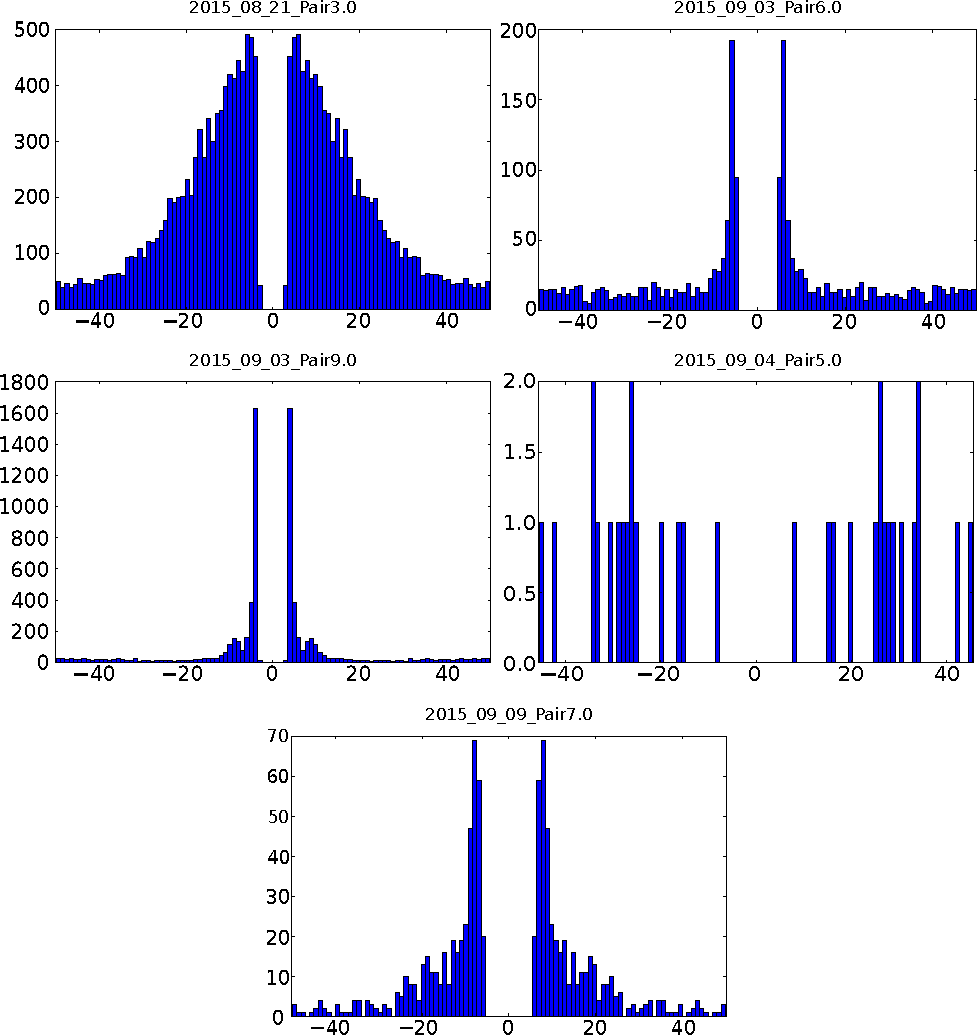
\includegraphics[width=\linewidth]{AC.pdf}
	\caption{Auto-Correlograms for all the recordings. The size of the bins in the histograms is 1 ms and the value for the lag is 50ms.
}
\label{fig:AC}
\end{figure}

All the auto-correlogram display a normal distribution, with a very consistent gap in the interval from -5ms to 5ms, assuring that the cell never spiked within 5ms of the previous, which conforms with the typical values of refractory period of 2-3ms.

It is worth noting that on the recording 939 the second peak is resolved around $\tau = -5 ms$ and $\tau = 5 ms$.

For each recording, phy was run with the following parameters:
The data was filtered with a forwards-backwards Butterworth filter of order 3 with cutoff frequency set to 500Hz. The noise standard deviation was evaluated in 50 excerpts of 1 second each. The weak threshold was $\theta_w = 2 \sigma_{noise}$ and the strong threshold was $\theta_s = 4.5 \sigma_{noise}$.

For each phy-detected spike, all electrodes whose corresponding mask value was non-zero were used.

In Fig. \ref{fig:CC} are the whole-probe cross-correlograms for the recordings.

\begin{figure}[!h]
	\centering
	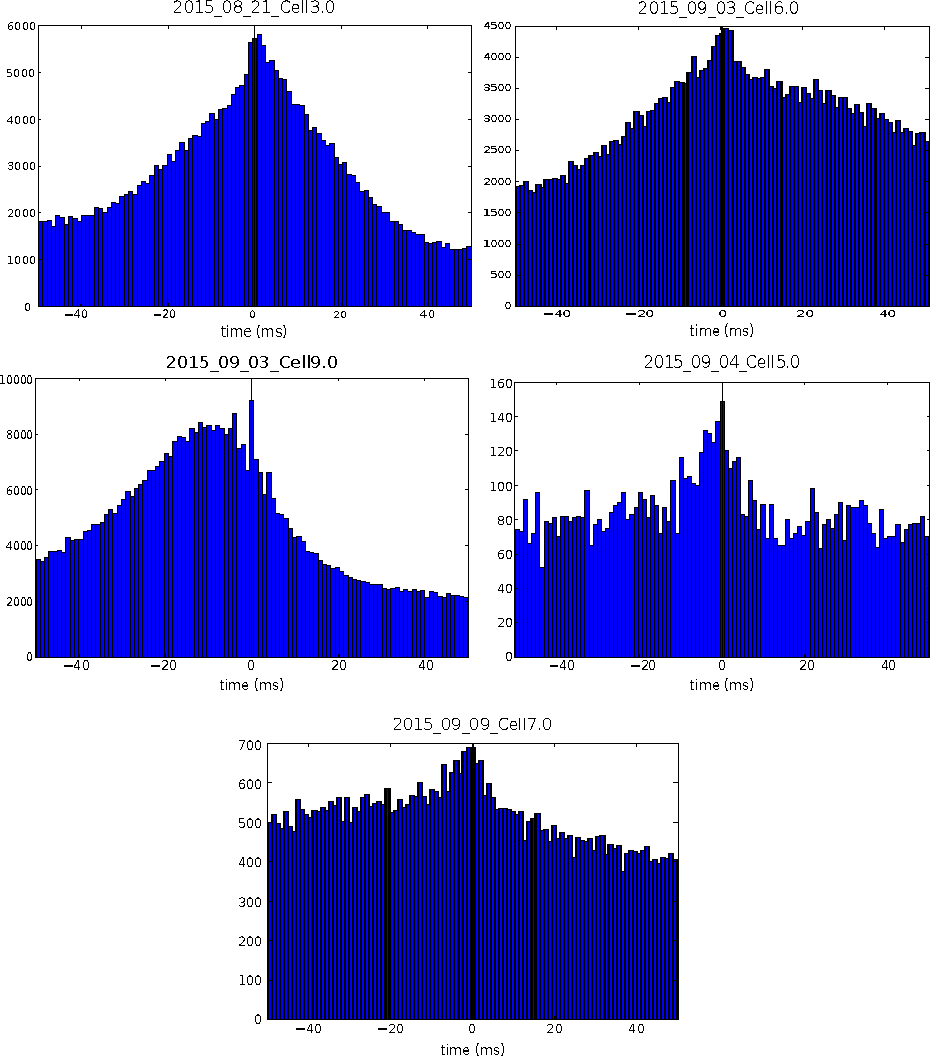
\includegraphics[width=\linewidth]{CC.pdf}
	\caption{Cross-Correlograms for all the recordings. The size of the bins in the histograms is 1 ms and the value for the lag is 50ms.
}
\label{fig:CC}
\end{figure}

In Appendix NUMBEROFAPPENDIX are the cross-correlograms per channel, where the spike train output by phy was splitted according to the electrode the spike was detected on using the masks.

\end{document}